\documentclass[11pt,a4paper]{article}

% Fonts: TeX Gyre Termes (Times equivalent) with matching math
\usepackage{fontspec}
\usepackage{unicode-math}
\setmainfont{texgyretermes}[
  Extension      = .otf,
  UprightFont    = *-regular,
  BoldFont       = *-bold,
  ItalicFont     = *-italic,
  BoldItalicFont = *-bolditalic,
]
\setmathfont{texgyretermes-math.otf}
\frenchspacing

% Body size / leading: 11.5pt / 13.5pt (matches GS manuscript class)
\makeatletter
\renewcommand{\@xpt}{11.5}
\renewcommand{\@xiipt}{13.5}
\renewcommand\normalsize{%
  \@setfontsize\normalsize\@xpt\@xiipt
  \abovedisplayskip 10\p@ \@plus2\p@ \@minus5\p@
  \abovedisplayshortskip \z@ \@plus3\p@
  \belowdisplayshortskip 6\p@ \@plus3\p@ \@minus3\p@
  \belowdisplayskip \abovedisplayskip
  \let\@listi\@listI}
\makeatother
\normalsize

% Page layout
\usepackage[margin=1in]{geometry}

% Math
\usepackage{amsmath,amsthm}

% Tables
\usepackage{array}
\usepackage{booktabs}
\setlength{\extrarowheight}{2pt}
\newcolumntype{L}[1]{>{\raggedright\arraybackslash}p{#1}}

% Float placement (forbid floats from migrating across section boundaries, GS-I convention)
\usepackage{float}
\usepackage[section]{placeins}

% Captions
\usepackage{caption}
\captionsetup{figurename=Fig.,labelsep=period,margin=1.2cm,labelfont=footnotesize}

% Lists (global spacing)
\usepackage{enumitem}
\setlist{leftmargin=1.2cm,labelindent*=.6cm,itemsep=0cm,parsep=0cm,topsep=0cm}

% Prevent orphaned headings
\usepackage{needspace}

% Section title formatting
\usepackage{titlesec}
\titleformat{\section}[block]{\fontsize{13pt}{15pt}\bfseries}{\thesection.}{0.6em}{}
\titlespacing*{\section}{0pt}{18pt}{8pt}
\titleformat{\subsection}[block]{\fontsize{11.5pt}{13.5pt}\bfseries\itshape}{\thesubsection.}{0.6em}{}
\titlespacing*{\subsection}{0pt}{14pt}{6pt}

% Graphics (for \scalebox on title-page divider glyph)
\usepackage{graphicx}

% TikZ + pgfplots (for in-document figures)
\usepackage{tikz}
\usetikzlibrary{positioning,arrows,calc}
\usepackage{pgfplots}
\pgfplotsset{compat=1.18}

% Paragraph formatting
\usepackage{indentfirst}
\emergencystretch=1em
\widowpenalty=10000
\clubpenalty=10000

% Float spacing
\setlength{\intextsep}{8pt plus 2pt minus 2pt}
\setlength{\floatsep}{8pt plus 2pt minus 2pt}
\setlength{\textfloatsep}{10pt plus 2pt minus 2pt}

% Display math spacing
\AtBeginDocument{%
  \setlength{\abovedisplayskip}{18pt plus 3pt minus 2pt}%
  \setlength{\belowdisplayskip}{18pt plus 3pt minus 2pt}%
  \setlength{\abovedisplayshortskip}{14pt plus 2pt minus 1pt}%
  \setlength{\belowdisplayshortskip}{14pt plus 2pt minus 1pt}%
}

% Table row spacing and font (harmonised with GS papers)
\renewcommand{\arraystretch}{1.05}
\AtBeginEnvironment{tabular}{\footnotesize}

% Typographic refinement
\usepackage{microtype}

% Footnotes pinned to page bottom (GS-I convention)
\usepackage[bottom]{footmisc}

% Superscript numeric citations
\usepackage[superscript,biblabel]{cite}

% Bibliography list geometry: superscript label sits in its own column,
% body text indents 1em past it, continuation lines hang-align under body.
\makeatletter
\renewenvironment{thebibliography}[1]
  {\section*{\refname}%
   \fontsize{10pt}{12pt}\selectfont
   \list{\@biblabel{\@arabic\c@enumiv}}%
        {\settowidth\labelwidth{\@biblabel{#1}}%
         \leftmargin\labelwidth
         \advance\leftmargin-0.8em
         \advance\leftmargin\labelsep
         \setlength\itemindent{1em}%
         \setlength\itemsep{6pt plus 1pt minus 1pt}%
         \setlength\parsep{0pt}%
         \usecounter{enumiv}%
         \let\p@enumiv\@empty
         \renewcommand\theenumiv{\@arabic\c@enumiv}}%
   \sloppy\clubpenalty4000\widowpenalty4000\sfcode`\.\@m}
  {\def\@noitemerr{\@latex@warning{Empty `thebibliography' environment}}%
   \endlist}
\makeatother

\usepackage{etoolbox}

% Pin abstract to 10pt/13pt with run-in "Abstract."
\renewenvironment{abstract}{%
  \fontsize{10pt}{13pt}\selectfont
  \begin{list}{}{%
    \setlength{\leftmargin}{0.5in}%
    \setlength{\rightmargin}{0.5in}%
    \setlength{\listparindent}{0pt}%
    \setlength{\parsep}{6pt plus 2pt minus 1pt}%
    \setlength{\topsep}{0pt}%
    \setlength{\partopsep}{0pt}%
  }\item[]\noindent\textbf{Abstract.}\hspace{0.5em}\ignorespaces
}{\end{list}}

% Colours
\usepackage{xcolor}

% Hyperlinks
\usepackage{hyperref}
\hypersetup{
  colorlinks=true,
  allcolors=blue!50!black,
  pdfauthor={K.R. Ryan},
  pdftitle={Parasitic Liquidity: Emission Extraction via Non-Functional Concentrated Liquidity Positions},
  pdfsubject={Concentrated liquidity gauge design and emission extraction},
  pdfkeywords={automated market maker, gauge design, DeFi security, mechanism design}
}

% Running header
\usepackage{fancyhdr}
\pagestyle{fancy}
\fancyhf{}
\fancyhead[L]{\small\itshape K.R.\ Ryan}
\fancyhead[R]{}
\fancyfoot[C]{\thepage}
\renewcommand{\headrulewidth}{0pt}
\fancypagestyle{plain}{%
  \fancyhf{}%
  \fancyfoot[C]{\thepage}%
  \renewcommand{\headrulewidth}{0pt}%
}

% Theorem environments (default amsthm styles)
\renewcommand\qedsymbol{\ensuremath{\mdlgblksquare}}
\theoremstyle{definition}
\newtheorem{definition}{Definition}
\theoremstyle{plain}
\newtheorem{theorem}{Theorem}
\newtheorem{lemma}{Lemma}
\newtheorem{proposition}{Proposition}
\newtheorem{corollary}{Corollary}

% Code block wrapper (use with \begin{verbatim}...\end{verbatim} inside)
\usepackage{mdframed}
\newenvironment{codeblock}{%
  \begin{mdframed}[%
    backgroundcolor=brown!3!white,%
    linewidth=0pt,%
    innertopmargin=6pt,%
    innerbottommargin=6pt,%
    innerleftmargin=12pt,%
    innerrightmargin=12pt,%
    leftmargin=0.075\linewidth,%
    rightmargin=0.075\linewidth,%
    skipabove=6pt,%
    skipbelow=6pt%
  ]\footnotesize%
}{%
  \end{mdframed}%
}

% Paragraph spacing (indented first line, no gap between paragraphs)
\setlength{\parindent}{18pt}
\setlength{\parskip}{0pt}

\begin{document}
\sloppy
\thispagestyle{plain}

\begin{center}
{\fontsize{10pt}{12pt}\selectfont WORKING PAPER}\\[6pt]
{\huge Parasitic Liquidity:\\[6pt]
Emission Extraction via Non-Functional\\[8pt]
Concentrated Liquidity Positions}

\vspace{14pt}
{\large K.R.\ Ryan}\\[4pt]
{\fontsize{9pt}{11pt}\selectfont Independent Researcher \quad|\quad ORCID - 0009-0004-6295-7040 \quad|\quad \href{mailto:gancor@gancor.xyz}{gancor@gancor.xyz}}\\[4pt]
{\fontsize{9pt}{11pt}\selectfont April 2026}

\vspace{12pt}
{\fontsize{9pt}{11pt}\selectfont
\begin{minipage}{0.82\linewidth}\centering
\textbf{Keywords}\hspace{0.6em}automated market maker \textperiodcentered\ gauge design \textperiodcentered\ DeFi security \textperiodcentered\ mechanism design\\[4pt]
\textbf{JEL:} G14, G19, G23, D47
\end{minipage}}
\end{center}

\vspace{-1pt}
\centerline{\scalebox{1.5}{$\therefore$}}
\vspace{14pt}

\begin{abstract}
This paper formalises \emph{parasitic liquidity}, an emission extraction strategy on concentrated liquidity DEXs that exploits a measurement gap between gauge accrual and swap facilitation. Three propositions establish that the Synthetix instantaneous stake accumulator used by Slipstream gauges and PancakeSwap's MasterChefV3 is memoryless in stake duration, independent of position width per unit of liquidity, and uncoupled from utilisation. Foundry suites against unmodified mainnet contracts on Base verify all three properties on both implementations. A point-in-time audit of one Aerodrome WETH/USDC pool found single-tick-width positions accounting for $63.4\%$ of in-range staked liquidity, with $92\%$ of sampled blocks containing zero swap events whilst those positions remained staked; a subsequent 14-day longitudinal scan of the same pool recorded $765{,}138$ mint events of which $98.6\%$ were one tick spacing wide. Across 31 daily anchors on the Aerodrome Slipstream VIRTUAL/WETH pool, the median operator capital floor for every-block-rebalance breakeven is \$11{,}223. Two gauge-level remediations, a minimum-width filter and a reward warmup, reduce parasitic effective yield by more than $99\%$ in combination against fork measured baselines analytically; a deployed partial fix (a 10-second emission cutoff) is shown analytically to leave 12--20 second cycles profitable in expectation, and width persistence is observed on the post-fix pools.
\end{abstract}

% ---- 1. Introduction ----
\section{Introduction}\label{sec:intro}

Uniswap V3 introduced concentrated liquidity, allowing LPs to specify a price range rather than providing liquidity across the full curve.\cite{adams2021} Only liquidity spanning the current tick is active for swaps. When protocols added emission incentives to this model, they needed a distribution mechanism. The solution adopted across ve(3,3) DEXs, PancakeSwap, and others was to distribute protocol native tokens to staked positions in proportion to their active liquidity.

The arrangement creates a measurement gap. Traders need swap depth that persists across price movements and absorbs order flow. Gauges reward instantaneous staked liquidity at a single point in time. The two quantities are different. In V2, liquidity along the constant-product curve is a single value $L=\sqrt{k}$ at every price, hence emissions distributed by LP token share is automatic emission distribution by tradeable depth. In V3, the active tick liquidity is the sum of $L$ values across heterogeneous positions, and the same emission formula no longer tracks depth. Section~\ref{sec:rootcause} visualises the lineage of the reward accumulator and the V2/V3 mechanism divergence.

The emission formula in a typical CL gauge is:
\begin{equation}\label{eq:gauge}
\text{reward}_i = \text{rewardRate} \times \Delta t \times \frac{L_i}{\sum_j L_j}
\end{equation}
where $L_i$ is position $i$'s liquidity at the active tick and the sum runs over all staked positions spanning that tick. This formula has three properties that together enable parasitic liquidity, each provable from the accumulator's update rule (Appendix~\ref{app:source}) and confirmed empirically in \S\ref{sec:foundry} (Table~\ref{tab:poc-results}).

\begin{proposition}[Memorylessness]\label{prop:warmup}
Let a Synthetix reward accumulator distribute emissions according to equation~\eqref{eq:gauge}. For any staked position $i$ with liquidity $L_i$ active at the tick over an interval $\Delta t$, the rewards accrued in that interval are $\text{rewardRate} \cdot \Delta t \cdot L_i / \sum_j L_j$, independent of the time elapsed since position $i$ was first staked. Equivalently, the per-unit-liquidity reward rate at any block depends on the present active tick state alone.
\end{proposition}

\begin{proposition}[Width independence]\label{prop:width}
Under the same accrual rule, for any two staked positions $i, j$ both active at the current tick over an interval $\Delta t$, $\text{reward}_i / \text{reward}_j = L_i / L_j$. The ratio is independent of the positions' tick-range widths $\Delta_i, \Delta_j$, including the boundary case in which one position spans a single tick spacing and the other spans an arbitrary number of tick spacings.
\end{proposition}

\begin{proposition}[No utilisation coupling]\label{prop:utilisation}
Under the same accrual rule, the rewards accrued by a position $i$ active at the tick over an interval $\Delta t$ depend only on $\Delta t$, $L_i$, and the active tick liquidity sum $\sum_j L_j$. They are independent of the number, direction, and total volume of swap events traversing position $i$'s range over the interval, including the case of zero swaps.
\end{proposition}

Together, the three propositions imply that a position can satisfy gauge staking requirements without serving any of the three quantities the gauge is intended to incentivise, namely sustained presence, range coverage, or trade facilitation.

This paper identifies parasitic liquidity as a distinct class of value extraction and traces its origin to the Synthetix reward accumulator (\S\ref{sec:definition}), formally characterises the profitability conditions (\S\ref{sec:analysis}), reports Foundry proof-of-concept suites against two independent protocol implementations on Base mainnet (\S\ref{sec:poc}), and proposes two remediation mechanisms with analysis of effectiveness and trade-offs (\S\ref{sec:remediation}). It sits within a broader programme on concentrated liquidity incentive design. Ryan\cite{ryan2026a,ryan2026b} characterises the geometric residual that arises on LP rebalancing under shared depositor balances; this paper analyses the emission-side analogue, where staked positions accrue gauge rewards without providing tradeable depth. A companion paper on constructive gauge design\cite{ryan2026c} addresses the protocol-side response, replacing $L_i$ in equation~\eqref{eq:gauge} with a scoring function whose factors track each of the three properties above.

% ---- 2. Related work ----
\section{Related work}\label{sec:related}

Documented MEV extraction classes operate at the swap layer. Daian \emph{et al.}\cite{daian2020} introduced miner extractable value (MEV) and surveyed the deployment of arbitrage and front-running bots in DEXs; Eskandari \emph{et al.}\cite{eskandari2019} systematise front-running attacks on blockchains into displacement, insertion and suppression categories, with case studies on early Ethereum DApps. Wan and Adams\cite{wan2022} and Capponi \emph{et al.}\cite{capponi2024} formalise just-in-time (JIT) liquidity, in which an LP mints a concentrated position immediately before a pending swap and burns it immediately after; Xiong \emph{et al.}\cite{xiong2023} measure 36{,}671 such attacks on Uniswap V3 and reframe JIT as an attack on passive LPs. Heimbach and Wattenhofer\cite{heimbach2022sok} systematise mitigations for transaction reordering manipulations, and Yang \emph{et al.}\cite{yang2022} provide a complementary taxonomy of MEV countermeasures.

Parasitic liquidity operates at the emission distribution layer rather than the swap layer. It does not require, depend on, or interact with any swap. Of the classes named above, the closest neighbour is JIT liquidity, which similarly mints and burns concentrated positions around individual events; JIT triggers on a pending swap in the mempool to capture its fees, whereas parasitic liquidity triggers on every block to capture emissions regardless of any swap activity (\S\ref{sec:distinct}).

A traditional finance analogue exists outside the AMM literature. Degryse \emph{et al.}\cite{degryse2020} document \emph{ghost liquidity} in equity markets, where high frequency liquidity providers post identical orders across multiple venues and cancel duplicates as soon as one fills; measured liquidity exceeds true tradeable liquidity. Parasitic liquidity is a DEX-specific instance of the same general pattern, where liquidity that satisfies the metric (instantaneous staked $L$ at the active tick) does not satisfy the underlying economic purpose (sustained tradeable depth).\footnote{0x have documented a contemporary sub-block analogue on Base's Flashblock architecture, where positions are minted for the duration of a single 200~ms sub-block to collect block-level LP rewards and withdrawn before swaps settle. See \url{https://0x.org/post/propamm-shenanigans}.}

Spearbit's November 2023 security review of Slipstream's concentrated liquidity implementation\cite{spearbit2023} noted that the reward accumulator may be gameable on chains with a mempool, described a claim-unstake-JIT-restake loop, and recommended evaluating whether a volume-based reward system would be fairer than the time-based accumulator; the issue was acknowledged with monitoring rather than redesign proposed. This paper formalises a more general strategy that does not require mempool visibility, applies cross-protocol on Slipstream and PancakeSwap MasterChefV3 (\S\ref{sec:foundry}), and provides aggregate on-chain evidence of use at scale (\S\ref{sec:onchain}).

Two deployed systems implement partial analogues of the remediations proposed in \S\ref{sec:remediation}. Algebra's eternal farming exposes an optional \texttt{minimalPositionWidth} parameter, used by QuickSwap on Polygon incentives at five times \texttt{tickSpacing}, a direct analogue of the minimum-width remediation. Merkl by Angle Labs\cite{merkl2023} distributes rewards off-chain via a time-weighted liquidity-contribution factor that rewards sustained concentration over time, a conceptual analogue of the warmup remediation. Both deployments predate this paper's formalisation of the underlying vulnerability.

% ---- 3. Parasitic Liquidity ----
\section{Parasitic liquidity}\label{sec:definition}

\subsection{Definition}\label{sec:def}

\begin{definition}[Parasitic Liquidity]
A concentrated liquidity position is parasitic if it satisfies the gauge's staking requirements without providing tradeable depth. The position is withdrawn and redeployed so frequently that it facilitates no swaps, yet it accrues emissions continuously.
\end{definition}

Let $\delta t$ denote the position's hold time per cycle and $\lambda$ the swap arrival rate on the target pool. A position is parasitic when:
\begin{equation}
\lambda \cdot \delta t \ll 1
\end{equation}

\subsection{Strategy}\label{sec:strategy}

A parasitic operator deploys a contract that executes the following loop each block:


\begin{codeblock}\begin{verbatim}
1. Read slot0() on target pool to obtain the current active tick t_c
2. Withdraw existing NFT from gauge
3. Decrease liquidity to zero, collect remaining tokens, burn NFT
4. Mint new NFT with tickLower = t_c, tickUpper = t_c + tickSpacing
5. Deposit new NFT into gauge
6. Repeat next block
\end{verbatim}\end{codeblock}


On L2 chains with block times of one to two seconds, this cycle completes every block, leaving the position perpetually at the current tick, at minimum width, and staked. Capital recycles each block with no lock up; the per-block impermanent loss exposure is bounded by hold time (Lemma~\ref{lem:ilratio}, \S\ref{sec:il}) and is several orders of magnitude smaller than per-block emission at observed pool volatility, but is not zero.

A cutoff-adapted variant runs the same loop on a multi-block cadence to satisfy any minimum-stake-time gate the gauge enforces. Width concentration is unchanged; only the rebalance frequency drops from once per block to once per minimum-stake-time interval.

\subsection{Root cause}\label{sec:rootcause}

The gauge reward formula in equation~\eqref{eq:gauge} is memoryless. A position staked in block $B$ immediately contributes to $\sum_j L_j$ and accrues its proportional share of emissions. When withdrawn in block $B+1$, it collects accrued rewards. The gauge retains no record of staking duration.

Synthetix introduced the reward accumulator pattern in \texttt{StakingRewards.sol} (2019) for fungible token staking. The core mechanism computes a global reward-per-token accumulator:


\begin{codeblock}\begin{verbatim}
function rewardPerToken() public view returns (uint256) {
    if (_totalSupply == 0) return rewardPerTokenStored;
    return rewardPerTokenStored.add(
        lastTimeRewardApplicable().sub(lastUpdateTime)
            .mul(rewardRate).mul(1e18).div(_totalSupply)
    );
}
\end{verbatim}\end{codeblock}


Each user's earned reward is the delta between the global accumulator and their last snapshotted value, multiplied by their stake. The pattern was designed for fungible ERC-20 staking where all participants provide an identical product.

\emph{Lineage.} Curve\cite{egorov2019} adopted this accumulator for gauge-weighted emissions in 2020, distributing CRV to LPs in proportion to their pool shares. Solidly (February~2022) forked Curve's gauges into the ve(3,3) model with permissionless gauge creation and fees-to-voters. A family of protocols refined this model: Velodrome (Optimism, June~2022), Thena (BNB~Chain, January~2023), Aerodrome (Base, August~2023), Ramses (Arbitrum), Pharaoh (Avalanche), Shadow (Sonic), and SwapX (Sonic).

\emph{V2 origin.} Earlier protocols in the lineage operated on constant product (V2) pools with fungible LP tokens. Figure~\ref{fig:v2} shows that a V2 LP token represented a proportional claim to the entire pool's liquidity curve. All LPs in a pool held proportional shares of the same single curve, so rewarding instantaneous stake was equivalent to rewarding sustained depth, and the instantaneous accumulator was appropriate. Later entrants adopted concentrated liquidity from launch, inheriting the same accumulator without revisiting its assumptions.

\definecolor{v2curve}{HTML}{1A535C}
\definecolor{v2fill}{HTML}{D8EAE7}
\begin{figure}[H]
\centering
\begin{tikzpicture}
\begin{axis}[
  width=0.56\linewidth, height=7.5cm,
  xlabel={$x$ reserve},
  ylabel={$y$ reserve},
  xmin=0, xmax=15, ymin=0, ymax=15,
  axis x line=bottom, axis y line=left,
  axis line style={black!55, line width=0.4pt, -},
  tick style={black!55, line width=0.4pt},
  ticks=none,
  every axis label/.style={font=\small},
  every tick label/.style={font=\footnotesize},
  xlabel style={yshift=-6pt},
  ylabel style={yshift=4pt},
  enlargelimits=false,
  clip=true
]
\addplot[draw=none, fill=v2fill, fill opacity=0.65, domain=0.05:15, samples=240] {10/x} \closedcycle;
\addplot[color=v2curve, line width=1.0pt, domain=0.05:15, samples=240] {10/x};
\draw[draw=v2curve, line width=0.4pt, dashed, opacity=0.55] (axis cs:1.4,0) -- (axis cs:1.4,7.14);
\draw[draw=v2curve, line width=0.4pt, dashed, opacity=0.55] (axis cs:3.16,0) -- (axis cs:3.16,3.16);
\draw[draw=v2curve, line width=0.4pt, dashed, opacity=0.55] (axis cs:7.14,0) -- (axis cs:7.14,1.4);
\draw[draw=black!70, line width=0.4pt, densely dotted, opacity=0.55] (axis cs:0,7.14) -- (axis cs:1.4,7.14);
\draw[draw=black!70, line width=0.4pt, densely dotted, opacity=0.55] (axis cs:0,3.16) -- (axis cs:3.16,3.16);
\draw[draw=black!70, line width=0.4pt, densely dotted, opacity=0.55] (axis cs:0,1.4) -- (axis cs:7.14,1.4);
\addplot[only marks, mark=*, mark size=2.4pt, color=v2curve]
  coordinates {(1.4,7.14) (3.16,3.16) (7.14,1.4)};
\node[font=\footnotesize, fill=white, draw=black!55, line width=0.4pt, inner sep=2.5pt, rounded corners=1pt, text=black!80]
  at (axis cs:2.6,8.4) {$L=\sqrt{k}$};
\node[font=\footnotesize, fill=white, draw=black!55, line width=0.4pt, inner sep=2.5pt, rounded corners=1pt, text=black!80]
  at (axis cs:3.9,4.0) {$L=\sqrt{k}$};
\node[font=\footnotesize, fill=white, draw=black!55, line width=0.4pt, inner sep=2.5pt, rounded corners=1pt, text=black!80]
  at (axis cs:7.9,2.4) {$L=\sqrt{k}$};
\node[font=\scriptsize, text=v2curve!75!black, anchor=south west]
  at (axis cs:0.9,13.4) {$y \to \infty$};
\node[font=\scriptsize, text=v2curve!75!black, anchor=south east]
  at (axis cs:14.4,0.95) {$x \to \infty$};
\node[font=\small\itshape, text=v2curve]
  at (axis cs:9.5,9.5) {$xy=k$};
\end{axis}
\end{tikzpicture}
\caption{Uniswap V2 constant-product curve $xy = k$.}\label{fig:v2}
\end{figure}

\emph{V3 break.} The design broke when these protocols grafted the same accumulator onto Uniswap~V3 position mechanics. Each V3 position is represented by a non-fungible token (NFT) with its own constant product invariant at its own $L$. Figure~\ref{fig:v3depth} contrasts the resulting per-position liquidity curves with the single curve V2 case: two positions with identical $L$ can provide vastly different tradeable depth depending on tick range width. The gauge formula rewards both at the same rate per unit of $L$, regardless of range, duration, or swap utilisation; the accumulator collapses the heterogeneous curves to scalar $L_i$ values when allocating emissions, treating non-fungible objects as if they were fungible LP shares.

\definecolor{widecol}{HTML}{4A90A4}
\definecolor{narrowcol}{HTML}{C0392B}
\definecolor{widefill}{HTML}{E0EBEF}
\definecolor{narrowfill}{HTML}{F5E0DD}
\begin{figure}[H]
\centering
\begin{tikzpicture}
\begin{axis}[
  width=0.56\linewidth, height=7.5cm,
  xlabel={virtual $x$ reserve},
  ylabel={virtual $y$ reserve},
  xmin=0, xmax=15, ymin=0, ymax=15,
  axis x line=bottom, axis y line=left,
  axis line style={black!55, line width=0.4pt, -},
  tick style={black!55, line width=0.4pt},
  ticks=none,
  every axis label/.style={font=\small},
  every tick label/.style={font=\footnotesize},
  xlabel style={yshift=-6pt},
  ylabel style={yshift=4pt},
  enlargelimits=false,
  clip=true
]
\addplot[draw=widecol!55, line width=0.6pt, dashed, domain=0.3:13.5, samples=120] {4/x};
\draw[dashed, line width=0.5pt, black!45] (axis cs:0,0) -- (axis cs:14.2,14.2);
\addplot[draw=widecol, fill=widefill, fill opacity=0.78, line width=1.6pt, domain=0.5:8, samples=160] {4/x} \closedcycle;
\addplot[draw=narrowcol!55, line width=0.6pt, dashed, domain=6.7:14.5, samples=80] {100/x};
\addplot[draw=narrowcol, fill=narrowfill, fill opacity=0.85, line width=1.6pt, domain=9.76:10.26, samples=40] {100/x} \closedcycle;
\addplot[only marks, mark=*, mark size=2.2pt, color=widecol] coordinates {(0.5,8) (8,0.5)};
\addplot[only marks, mark=*, mark size=2.2pt, color=narrowcol] coordinates {(9.76,10.25) (10.26,9.75)};
\addplot[only marks, mark=square*, mark size=1.8pt, color=widecol] coordinates {(2,2)};
\addplot[only marks, mark=square*, mark size=1.8pt, color=narrowcol] coordinates {(10,10)};
\node[font=\footnotesize\bfseries, text=widecol, anchor=west]
  at (axis cs:2.4,1.9) {$L_w = 2$};
\node[font=\footnotesize\bfseries, text=narrowcol, anchor=west]
  at (axis cs:10.4,9.9) {$L_n = 10$};
\node[font=\scriptsize\bfseries, text=black!85, anchor=east]
  at (axis cs:13.0,13.3) {active price $P$};
\end{axis}
\end{tikzpicture}
\caption{Two V3 positions in virtual reserves space, with the wide-range position drawn in blue and the narrow-range position drawn in red. Each position's $xy = L_i^2$ invariant is solid within its tick range and dashed beyond.}\label{fig:v3depth}
\end{figure}

PancakeSwap's MasterChefV3 arrived at the same vulnerability via parallel evolution, applying the Synthetix accumulator (used since MasterChef~V1) to their Uni~V3 fork. Any protocol that distributes emissions under this accumulator pattern on a concentrated liquidity pool is exposed to the same extraction mechanism. Figure~\ref{fig:accumulator} contrasts the pattern's V2 and V3 applications.

\begin{figure}[H]
\centering
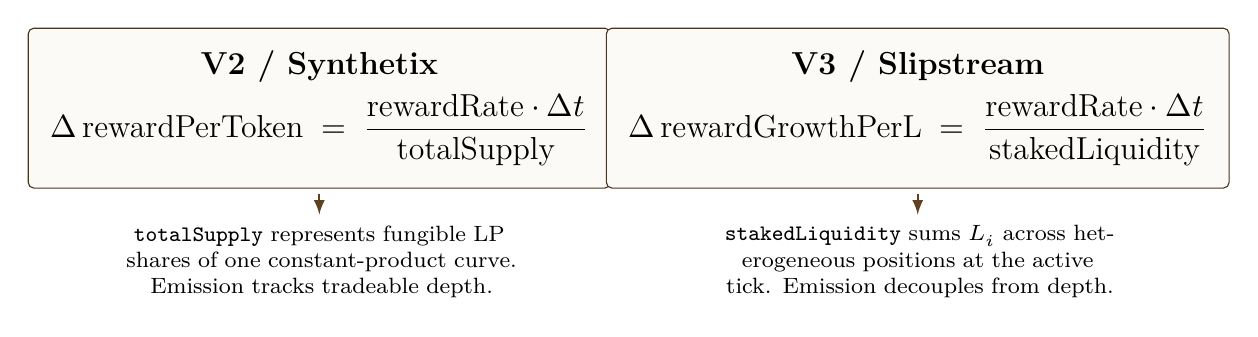
\begin{tikzpicture}[
  >=latex,
  box/.style={
    draw=brown!40!black, fill=brown!4, rounded corners=2pt,
    inner sep=8pt, align=center, minimum width=6.2cm, minimum height=1.8cm
  },
  outcome/.style={font=\footnotesize, align=center, text width=6cm},
  arrow/.style={->, thick, brown!50!black, shorten >=2pt, shorten <=2pt}
]
\node[box] (v2) at (-3.8cm, 0) {%
  \textbf{V2 / Synthetix}\\[3pt]
  $\Delta\,\text{rewardPerToken} \;=\; \dfrac{\text{rewardRate} \cdot \Delta t}{\text{totalSupply}}$
};
\node[box] (v3) at (3.8cm, 0) {%
  \textbf{V3 / Slipstream}\\[3pt]
  $\Delta\,\text{rewardGrowthPerL} \;=\; \dfrac{\text{rewardRate} \cdot \Delta t}{\text{stakedLiquidity}}$
};
\draw[arrow] (v2.south) -- ++(0,-0.4);
\draw[arrow] (v3.south) -- ++(0,-0.4);
\node[outcome] at (-3.8cm, -1.95) {%
  \texttt{totalSupply} represents fungible LP shares of one constant-product curve. Emission tracks tradeable depth.
};
\node[outcome] at (3.8cm, -1.95) {%
  \texttt{stakedLiquidity} sums $L_i$ across heterogeneous positions at the active tick. Emission decouples from depth.
};
\end{tikzpicture}
\caption{The Synthetix reward-accumulator pattern in V2 and V3.}\label{fig:accumulator}
\end{figure}

In Slipstream derived gauges, the reward growth update divides the per-block reward by the total active liquidity across all staked positions at the current tick. PancakeSwap's V3 liquidity mining pool performs the same operation against its own staked liquidity counter. Full source listings for both functions, including the specific accumulator lines, are reproduced in Appendix~\ref{app:source}.


% ---- 4. Formal Analysis ----
\section{Formal analysis}\label{sec:analysis}

\subsection{Profitability condition}\label{sec:profit}

\noindent\emph{Notation.} The symbols used in this section and \S\S\ref{sec:capeff}--\ref{sec:capitalfloor} are summarised in Table~\ref{tab:notation} (Appendix~\ref{app:notation}).

\noindent\emph{Setup.} Let $E$ be the per second USD emission to the pool, $L_{\text{op}}$ the parasitic operator's position liquidity, $L_p$ the total in-range pool liquidity at the current tick, $f$ the rebalance frequency, and $g$ the gas cost per cycle.

\noindent\emph{Revenue per second.}
\begin{equation}
R = E \cdot \frac{L_{\text{op}}}{L_p}
\end{equation}

\noindent\emph{Cost per second.}
\begin{equation}
C = f \cdot g
\end{equation}

\noindent\emph{Profitability condition.}
\begin{equation}
E \cdot \frac{L_{\text{op}}}{L_p} > f \cdot g
\end{equation}

On Base (two-second blocks, sub-cent gas), with $g \approx \$0.005$ per rebalance cycle and one rebalance per block:
\begin{equation}
C = \frac{0.005}{2} = \$0.0025/\text{sec} = \$216/\text{day}
\end{equation}

A small amount of capital can dominate the liquidity share at the active tick, and an operator targeting multiple pools amortises the fixed gas cost across them.

\subsection{Capital efficiency}\label{sec:capeff}

Each rebalance cycle withdraws and redeploys the full principal, so the operator's capital is never locked. The effective capital requirement is a single position plus gas reserves. Legitimate LPs, by contrast, keep capital deployed and exposed to impermanent loss for the duration of their position.

\subsection{Fee income versus emission income}\label{sec:feevemission}

A single-tick position minted at the current tick covers one tick spacing for one block. The point-in-time audit in \S\ref{sec:onchain} found that in $92\%$ of sampled blocks on the audited pool, the position was staked through zero \texttt{Swap} events. In those blocks the operator earned emissions only, and the breakeven analysis in \S\ref{sec:profit} and the capital floor analysis in \S\ref{sec:capitalfloor} already clear at the emission-only level. Fee income in the remaining blocks is upside rather than subsidy. The strategy's profitability does not depend on it.

\subsection{Dilution of legitimate liquidity providers}\label{sec:dilution}

Legitimate LPs receive a reduced fraction of emissions:
\begin{equation}
\frac{L_{\text{legit}}}{L_{\text{legit}} + L_{\text{op}}}
\end{equation}

Single-tick-width positions concentrate all capital into one tick spacing. For small tick ranges, liquidity scales inversely with range width, so the same capital in one tick spacing produces roughly ten times the liquidity of the same capital spread across ten spacings. A small amount of capital can therefore dominate the liquidity share at the active tick and capture a disproportionate fraction of emissions.

\subsection{Scalability}\label{sec:scale}

The parasitic share of emissions scales linearly with the number of operators:
\begin{equation}
\text{Parasitic share} = \frac{n \cdot L_{\text{op,avg}}}{L_{\text{legit}} + n \cdot L_{\text{op,avg}}}
\end{equation}

Nothing in the protocol prevents multiple operators from targeting the same pool. As $n$ increases, legitimate LP share approaches zero. The low capital requirement (\S\ref{sec:capeff}) and sub-cent gas costs on L2s make the barrier to entry negligible.

\subsection{Cross-chain affordability}\label{sec:affordability}

The Base example above is unusually permissive, with 0.005~gwei base fees, two-second blocks, and high-density gauge emissions. Other chains run on different cost structures, and the profitability condition $E \cdot L_{\text{op}}/L_p > g/T_{\text{block}}$ has different solutions on each. Figure~\ref{fig:affordability} plots gas cost per rebalance cycle against per-block pool emission for eighteen gauged CL pools across four chains (eight Aerodrome on Base, seven PancakeSwap V3 on BSC, one Ramses V2 on Arbitrum, two Shadow on Sonic). Polygon's QuickSwap V3 sample returned zero accumulator growth across the window and is omitted from the figure.

\definecolor{regionprof}{HTML}{E0EFE5}
\definecolor{regionmarg}{HTML}{F5EFD8}
\definecolor{regionunprof}{HTML}{F4DDDB}
\definecolor{chainpoint}{HTML}{1A3554}
\definecolor{ccBase}{HTML}{1A535C}
\definecolor{ccBSC}{HTML}{C0392B}
\definecolor{ccArb}{HTML}{4A90A4}
\definecolor{ccSonic}{HTML}{E67E22}

\begin{figure}[H]
\centering
\begin{tikzpicture}
\begin{axis}[
  width=0.85\linewidth, height=8cm,
  xlabel={Gas cost per rebalance cycle (USD)},
  ylabel={Per-block pool emission (USD)},
  xmode=log, log basis x=10,
  ymode=log, log basis y=10,
  xmin=0.0005, xmax=20, ymin=0.00001, ymax=20,
  axis x line=bottom, axis y line=left,
  axis line style={black!55, line width=0.4pt, -},
  tick style={black!55, line width=0.4pt},
  every axis label/.style={font=\small},
  every tick label/.style={font=\footnotesize},
  xlabel style={yshift=-6pt},
  ylabel style={yshift=4pt},
  xtick={0.001,0.01,0.1,1,10},
  xticklabels={\$0.001,\$0.01,\$0.10,\$1,\$10},
  ytick={0.00001,0.0001,0.001,0.01,0.1,1,10},
  yticklabels={\$10\textsuperscript{-5},\$10\textsuperscript{-4},\$0.001,\$0.01,\$0.10,\$1,\$10},
  enlargelimits=false,
  clip=true
]
\path[fill=regionprof]
  (axis cs:0.0005, 0.005) --
  (axis cs:2, 20) --
  (axis cs:0.0005, 20) -- cycle;
\path[fill=regionmarg]
  (axis cs:0.0005, 0.00001) --
  (axis cs:0.00001, 0.00001) --
  (axis cs:20, 20) --
  (axis cs:2, 20) --
  (axis cs:0.0005, 0.005) -- cycle;
\path[fill=regionunprof]
  (axis cs:0.00001, 0.00001) --
  (axis cs:20, 20) --
  (axis cs:20, 0.00001) -- cycle;
\addplot[draw=black!50, line width=0.5pt, dashed, samples=2, domain=0.00001:20] {x};
\addplot[draw=black!50, line width=0.5pt, densely dotted, samples=2, domain=0.0005:2] {10*x};
% v08 expanded sample: per-chain whisker (min..max) + filled median + hollow circle per pool.
% Pool counts: Base 8, BSC 7, Arbitrum 1, Sonic 2. Polygon empirically zero (annotated).
% Source: scripts/data/v08_per_pool_summary.csv (auto-generated via v08-figure.py).
\addplot[no marks, color=ccBase, line width=1.0pt] coordinates {(0.008286, 6.2e-05) (0.008286, 0.54852)};
\addplot[only marks, mark=o, mark size=1.8pt, color=ccBase] coordinates {(0.008286, 0.54852) (0.008286, 0.40216) (0.008286, 0.080953) (0.008286, 0.0041) (0.008286, 0.001197) (0.008286, 0.004106) (0.008286, 0.001635) (0.008286, 6.2e-05)};
\addplot[only marks, mark=*, mark size=2.6pt, color=ccBase] coordinates {(0.008286, 0.004103)};
\addplot[no marks, color=ccBSC, line width=1.0pt] coordinates {(0.52598, 0.001262) (0.52598, 0.013906)};
\addplot[only marks, mark=o, mark size=1.8pt, color=ccBSC] coordinates {(0.52598, 0.013906) (0.52598, 0.004373) (0.52598, 0.003086) (0.52598, 0.001353) (0.52598, 0.002706) (0.52598, 0.001752) (0.52598, 0.001262)};
\addplot[only marks, mark=*, mark size=2.6pt, color=ccBSC] coordinates {(0.52598, 0.002706)};
\addplot[only marks, mark=*, mark size=2.6pt, color=ccArb] coordinates {(0.082707, 1.9e-05)};
\addplot[only marks, mark=o, mark size=1.8pt, color=ccArb] coordinates {(0.082707, 1.9e-05)};
\addplot[no marks, color=ccSonic, line width=1.0pt] coordinates {(0.000629, 0.002836) (0.000629, 0.005132)};
\addplot[only marks, mark=o, mark size=1.8pt, color=ccSonic] coordinates {(0.000629, 0.005132) (0.000629, 0.002836)};
\addplot[only marks, mark=*, mark size=2.6pt, color=ccSonic] coordinates {(0.000629, 0.003984)};
\node[font=\footnotesize, text=ccBase,  anchor=south west] at (axis cs:0.0095, 0.54852)  {Base ($N{=}8$)};
\node[font=\footnotesize, text=ccBSC,   anchor=south west] at (axis cs:0.55,   0.013906) {BSC ($N{=}7$)};
\node[font=\footnotesize, text=ccArb,   anchor=south west] at (axis cs:0.095,  1.9e-05)  {Arbitrum ($N{=}1$)};
\node[font=\footnotesize, text=ccSonic, anchor=south west] at (axis cs:0.0008, 0.005132) {Sonic ($N{=}2$)};
\node[font=\scriptsize\itshape, text=green!50!black] at (axis cs:0.0025, 6) {profitable};
\node[font=\scriptsize\itshape, text=yellow!40!black] at (axis cs:0.4, 0.7) {marginal};
\node[font=\scriptsize\itshape, text=red!50!black] at (axis cs:6, 0.0005) {unprofitable};
\node[font=\scriptsize, text=black!55, anchor=south west] at (axis cs:0.7, 7) {$10\%$ share};
\node[font=\scriptsize, text=black!55, anchor=south west] at (axis cs:6, 7) {$100\%$ share};
\end{axis}
\end{tikzpicture}
\caption{Cross-chain affordability of parasitic strategies, 31 daily anchors over March 2026. Hollow circles are per pool emission medians; filled markers are per chain medians; bars span the per chain min-to-max range. Diagonal lines mark breakeven at $10\%$ and $100\%$ parasitic share.}\label{fig:affordability}
\end{figure}

\emph{Gas.} Per day gas at each anchor is the on-chain \texttt{baseFeePerGas} (a flat 1~gwei on BSC, which does not expose the EIP-1559 base fee) times a per chain Foundry-calibrated rebalance-cycle gas estimate and the day's CoinGecko USD price for the native token.

\emph{Enumeration.} V3 CL pools are enumerated per chain via the canonical V3 factory's \texttt{PoolCreated} event log: 3{,}308 Aerodrome pools on Base, 84 PancakeSwap V3 pools on BSC with non-zero MasterChefV3 allocation, 44 Arbitrum pools mapped from Ramses voter \texttt{DistributeReward}-emitted gauges, two known Shadow pools on Sonic seeded manually (the Shadow factory and voter route events through inaccessible internal deployers), and 7{,}325 Polygon Algebra pools. Each pool then passes a filter requiring an attached gauge at the first March anchor, a non-zero reward rate on at least 10 of 31 anchors, a median emission above $10^{-7}$ USD per block, and a median in-range pool liquidity $L_p$ above $10^{10}$.

\emph{Scoring.} Surviving pools are scored on four orthogonal dimensions and the top three per bucket per chain are taken with deduplication. Bucket~A ranks by median per block emission $E_{\text{block}}$. Bucket~B ranks by $E_{\text{block}} / L_p$, surfacing pools where the active tick denominator is small enough that a modest position dominates the gauge share. Bucket~C ranks by $E_{\text{block}} / V_{\text{ir}}$, where $V_{\text{ir}}$ is the swap volume whose post-swap tick lies within $\pm 5 \times \text{tickSpacing}$ of the day's median tick. Bucket~D combines all three as the composite $E_{\text{block}} / (L_p \cdot \sqrt{V_{\text{ir}}})$. To prevent the last three buckets from selecting on incentive dust, they are restricted to pools whose median emission exceeds \$0.001 per block on Base, BSC, and Sonic; Arbitrum is not floor restricted because the RAM reward token's collapsed market value would exclude every Ramses pool on absolute USD criteria.

The final sample contains eight Base pools, seven BSC pools, one Arbitrum pool (Ramses' WETH/USDC, the only candidate to survive the gauge decay threshold from 44), two Sonic pools, and zero Polygon pools.

\begin{table}[H]
\centering
\caption{Cross-chain pool affordability medians, 31 daily anchors, March 2026.}\label{tab:poolaffordability}

\textbf{Base} -- Aerodrome Slipstream, gas \$0.0083/cycle, 8 sampled pools \\[2pt]
\begin{tabular}{@{}l r r r@{}}
\toprule
Pool & Tick spacing & Emission \$/block & Breakeven share \\
\midrule
\multicolumn{4}{@{}l}{Profitable for an extractor with realistic capture} \\
\quad {\scriptsize\emph{WETH/USDC}}     & 100 & 0.549   & 1.51\%  \\
\quad {\scriptsize\emph{WETH/VVV}}      & 100 & 0.402   & 2.06\%  \\
\addlinespace[2pt]
\multicolumn{4}{@{}l}{Marginal (between the $10\%$ and $100\%$ lines in Figure~\ref{fig:affordability})} \\
\quad {\scriptsize\emph{WETH/AERO}}     & 200 & 0.081   & 10.24\% \\
\addlinespace[2pt]
\multicolumn{4}{@{}l}{Unprofitable (gas exceeds $100\%$ capture of in-range emission)} \\
\quad {\scriptsize\emph{tBTC/USDC}}     & 200 & 0.0041  & 202\%   \\
\quad {\scriptsize\emph{WETH/bsdETH}}   & 1   & 0.0041  & 202\%   \\
\quad {\scriptsize\emph{tBTC/WETH}}     & 200 & 0.0016  & 507\%   \\
\quad {\scriptsize\emph{WETH/USD+}}     & 100 & 0.0012  & 692\%   \\
\addlinespace[2pt]
\multicolumn{4}{@{}l}{Floor-fill outlier (below the bucket-D emission threshold)} \\
\quad {\scriptsize\emph{PSTAKE/USDC}}   & 200 & $6.2{\times}10^{-5}$ & 13{,}361\% \\
\bottomrule
\end{tabular}

\vspace{8pt}

\textbf{Other chains} -- chain-level summary \\[2pt]
\begin{tabular}{@{}l l r r l l@{}}
\toprule
Chain & Protocol & Gas/cycle & Pools & Breakeven range & Verdict \\
\midrule
BSC      & PancakeSwap V3 & \$0.526   & 7 & $38{\times}$ to $417{\times}$ pool L & unprofitable \\
Arbitrum & Ramses V2      & \$0.083   & 1 & $4{,}341{\times}$ pool L            & unprofitable \\
Sonic    & Shadow         & \$0.0006  & 2 & 12\% to 22\%                        & marginal \\
\bottomrule
\end{tabular}
\end{table}

Base concentrates the strategy's profitability in two headline incentive pairs (WETH/USDC and WETH/VVV) at 1.5--2\% of pool L, with WETH/AERO at 10\% sitting on the boundary of the marginal band. The next four pools (tBTC/USDC, WETH/bsdETH, tBTC/WETH, WETH/USD+) require capture between two and seven times the in-range L: their per-block emission is too thin to clear gas even at 100\% gauge share, so the pool is not extractable at every-block cadence regardless of capital. The PSTAKE/USDC floor-fill outlier confirms that pools below the bucket-D emission threshold of \$0.001 per block are uneconomic regardless of how favourable their liquidity or volume profile looks on the composite ratio; sampling without an absolute floor would surface incentive dust as false positives.

The other three chains in the cross-chain summary land at chain-level verdicts. BSC's seven sampled pools span a 12$\times$ emission range, yet all require 38$\times$ to 417$\times$ pool L to break even; the infeasibility is genuinely chain-driven by gas cost rather than a low-allocation pool-choice artefact. Arbitrum's surviving Ramses pool, the only one that cleared the 10-of-31-emitting-days filter from 44 candidates, sits 4{,}341$\times$ pool L away from breakeven because the RAM reward token has collapsed in market value. Sonic's two Shadow pools clear the marginal band at 12\% to 22\% of pool L. Polygon's expanded probe of the first 50 of 7{,}325 QuickSwap V3 pools at the March 1 anchor returned zero \texttt{activeIncentive} pointers, consistent with a dormant gauge program for the window; the chain is omitted from the table because there is no surviving sample to display.

The vulnerability holds wherever the Synthetix accumulator runs on concentrated liquidity, but extraction is currently economically viable only on a narrow set of cheap-gas, dense-emission L2s. Both inputs are governance- and market-determined, so a chain below the breakeven line today can move into the profitable region with a single emission-vote outcome or a sustained drop in gas prices.

\subsection{Active-tick capital floor}\label{sec:capitalfloor}

Figure~\ref{fig:affordability} expressed parasitic affordability as a fraction of pool liquidity. On a V3/Slipstream pool the meaningful denominator is the \emph{active-tick} liquidity returned by \texttt{pool.liquidity()}, rather than the sum over all staked positions. Reframing in those terms produces a USD capital floor for an operator who deploys a one-tick-spacing-wide position centred on the active tick and rebalances every block.

The breakeven inequality for an operator with position liquidity $L_{\text{op}}$ at the active tick and an every-block rebalance schedule is
\begin{equation}
\frac{L_{\text{op}}}{L_p} \cdot E_{\text{block}} \;>\; g,
\label{eq:floor}
\end{equation}
where $L_p$ is the total in-range pool liquidity, $E_{\text{block}}$ is per-block USD emission, and $g$ is per-cycle USD gas cost. Solving for $L_{\text{op}}$ and converting to USD via the canonical Uniswap V3 amounts formula at a position width of one tick spacing yields the closed-form result below.

\begin{corollary}[Capital Floor]\label{cor:capitalfloor}
Let a CL gauge satisfy Propositions~\ref{prop:warmup}--\ref{prop:utilisation} on a pool with active-tick liquidity $L_p$ and per-block USD emission $E_{\text{block}}$ at a given block, and let $g$ denote the per-cycle USD gas cost of a rebalance at that block. For an operator rebalancing every block at the active tick over a one-tick-spacing range, the breakeven operator capital is
\begin{equation}
C^{*} \;=\; \frac{g \cdot L_p \cdot V_{\text{per-L}}}{E_{\text{block}}},
\label{eq:capfloor}
\end{equation}
where $V_{\text{per-L}}$ is the USD value of unit-$L$ at a one-tick-spacing range centred on the active tick, computed via the canonical Uniswap V3 amount equations.
\end{corollary}

\begin{proof}
By Proposition~\ref{prop:utilisation}, the operator's per-block reward depends only on $\Delta t$, $L_{\text{op}}$, and $L_p$. By Proposition~\ref{prop:warmup}, the operator earns at full per-unit-liquidity rate from the first block of stake, so the rebalance cycle pays out $L_{\text{op}}/L_p \cdot E_{\text{block}}$ regardless of how recently the position was minted. By Proposition~\ref{prop:width}, the per-$L$ rate is independent of position range width, so the operator may freely choose the tightest valid range without yield penalty. Substituting into~\eqref{eq:floor} and solving for $L_{\text{op}}$ gives $L_{\text{op}}^{*} = g L_p / E_{\text{block}}$. Converting $L_{\text{op}}^{*}$ to USD via the canonical Uniswap V3 amount formulas at a one-tick-spacing range centred on the active tick (which produces $V_{\text{per-L}}$ by definition) gives~\eqref{eq:capfloor}.
\end{proof}

Figure~\ref{fig:capitalfloor} plots the resulting daily capital floor and the implied active-tick capital ($L_p \cdot V_{\text{per-L}}$, a lower bound on dollars actually contributing to active-tick rewards) for the Aerodrome Slipstream VIRTUAL/WETH CL100 pool over the same 31-day window. Across the window the capital floor has a median of \$11{,}223, an interquartile range of \$7{,}908--\$15{,}709, and an absolute range of \$2{,}306--\$37{,}743. Implied active-tick capital ranges from \$16{,}069 to \$153{,}352 across the window. Every quantity in this calculation is read directly from on-chain state at each anchor block. Pool liquidity and sqrt price come from the Slipstream pool getters \texttt{liquidity()} and \texttt{slot0()}, the emission rate from the gauge's \texttt{rewardRate()}, and the gas component from the JSON-RPC \texttt{baseFeePerGas} field. No assumption about transaction ordering, sub-block reordering, sequencer behaviour, or MEV is required.

\definecolor{flcol}{HTML}{B43D3F}
\definecolor{tvlcol}{HTML}{1A3554}
\definecolor{medcol}{HTML}{707070}

\begin{figure}[H]
\centering
\begin{tikzpicture}
\begin{axis}[
  width=0.92\linewidth, height=7.2cm,
  xlabel={Day in March 2026 (anchor at 12:00 UTC)},
  ylabel={USD},
  ymode=log, log basis y=10,
  xmin=0.5, xmax=31.5, ymin=1500, ymax=400000,
  axis x line=bottom, axis y line=left,
  axis line style={black!55, line width=0.4pt, -},
  tick style={black!55, line width=0.4pt},
  every axis label/.style={font=\small},
  every tick label/.style={font=\footnotesize},
  xlabel style={yshift=-6pt},
  ylabel style={yshift=4pt},
  xtick={1,5,10,15,20,25,31},
  ytick={2000,5000,10000,20000,50000,100000,200000},
  yticklabels={\$2k,\$5k,\$10k,\$20k,\$50k,\$100k,\$200k},
  legend style={at={(0.98,0.98)}, anchor=north east, font=\scriptsize, draw=black!40, fill=white, line width=0.3pt},
  enlargelimits=false,
  clip=true
]
\addplot[draw=tvlcol, line width=0.6pt, mark=square*, mark size=1.2pt] coordinates {
  (1,103145) (2,71048) (3,112187) (4,79295) (5,37340)
  (6,32844)  (7,86091) (8,32468)  (9,97895) (10,23537)
  (11,62197) (12,131439) (13,66495) (14,153352) (15,35859)
  (16,145628) (17,136198) (18,58518) (19,35121) (20,91377)
  (21,39657) (22,110314) (23,99642) (24,64015) (25,69157)
  (26,112099) (27,79084) (28,88432) (29,53736) (30,85268)
  (31,16069)
};
\addlegendentry{Implied active-tick capital ($L_p \cdot V_{\text{per-L}}$)}
\addplot[draw=flcol, line width=0.7pt, mark=*, mark size=1.4pt] coordinates {
  (1,11223) (2,7908)  (3,14258) (4,9202)  (5,5583)
  (6,5031)  (7,13281) (8,5079)  (9,15709) (10,3795)
  (11,9598) (12,19797) (13,10057) (14,24155) (15,5601)
  (16,23564) (17,22239) (18,10508) (19,8138) (20,20840)
  (21,9203) (22,25635) (23,37743) (24,14133) (25,15280)
  (26,15515) (27,10800) (28,12104) (29,7266) (30,11888)
  (31,2306)
};
\addlegendentry{Operator capital floor (every-block breakeven)}
\addplot[draw=medcol, line width=0.4pt, dashed, samples=2, domain=0.5:31.5] {11223};
\node[font=\scriptsize, text=medcol, anchor=south east] at (axis cs:31.4, 11223) {median floor \$11.2k};
\end{axis}
\end{tikzpicture}
\caption{Daily operator capital floor for active-tick parasitic profitability on Aerodrome Slipstream VIRTUAL/WETH (CL100), at 12:00 UTC anchors over 1--31 March 2026.}\label{fig:capitalfloor}
\end{figure}

The day 31 trough reflects a transient drop in active-tick $L_p$ at the 12:00~UTC anchor, where \texttt{pool.liquidity()} fell by roughly 80\% from the previous day's anchor whilst $V_{\text{per-L}}$ was unchanged; the floor returns to the typical four-figure band across the rest of the window.

Across every day in the window, an operator deploying between \$2{,}300 and \$37{,}700 at the active tick breaks even rebalancing every block. The audited WETH/USDC pool in \S\ref{sec:onchain} carries a single-tick gauge share of $63.4\%$, sitting orders of magnitude above the floor in Figure~\ref{fig:capitalfloor}. Equation~\eqref{eq:floor} clears at four-figure capital from accumulator economics alone, with no assumption about sub-block ordering, sequencer behaviour, or MEV amplification.

\subsection{Impermanent loss exposure}\label{sec:il}

A common framing of single-block-rebalance operators is that they carry impermanent loss like any other liquidity provider. The framing collapses a quantitative comparison into a binary one. An operator who holds a position for a single Base block is exposed for two seconds per cycle; a legitimate LP at the same width is exposed for the full duration of their hold.

For an in-range concentrated liquidity position with annualised realised volatility $\sigma$ and hold duration $t$, the expected impermanent loss is approximated by
\begin{equation}
\text{IL}/V \;\approx\; \tfrac{1}{8}\,\sigma^{2}\,(t / T_{\text{yr}}),
\label{eq:il}
\end{equation}
where $T_{\text{yr}}$ is seconds per year. The expression is exact for full-range positions and a tight upper bound for narrow CL positions whilst in range (Loesch \emph{et al.}\cite{loesch2021}). Linearity in $t$ at fixed $\sigma$ is the relevant property here, and yields the following volatility-independent ratio.

\begin{lemma}[IL Hold-Time Linearity]\label{lem:ilratio}
Under the in-range CL impermanent-loss approximation~\eqref{eq:il}, two positions at identical width and active tick that remain in range over hold durations $t_1$ and $t_2$ satisfy
\[
\frac{\mathrm{IL}_2}{\mathrm{IL}_1} \;=\; \frac{t_2}{t_1},
\]
independent of the realised volatility $\sigma$.
\end{lemma}

\begin{proof}
Direct from~\eqref{eq:il}: $\mathrm{IL}_i / V \approx \tfrac{1}{8} \sigma^2 (t_i / T_{\text{yr}})$ for $i \in \{1, 2\}$. Taking the ratio cancels both $V$ and $\sigma^2$, leaving $t_2/t_1$.
\end{proof}

Across the same 31-day March 2026 window used in \S\ref{sec:capitalfloor}, realised annualised volatility on a Base-native token-pair ratio (used as a proxy for the cited pool) had a median of 45\% with a daily range of 39\%--53\%.\footnote{Standard deviation of daily log-returns on the AERO/WETH ratio, rolling 30-day window, annualised by $\sqrt{365}$. The operator-vs-legitimate IL ratio is hold-time-only and therefore independent of the volatility series chosen; only the absolute IL levels in Table~\ref{tab:il-ratios} depend on it.} Table~\ref{tab:il-ratios} reports the median per-hold IL exposure for the parasitic operator and three reference legitimate-LP profiles, plus the ratio of legitimate-LP exposure to operator exposure.

\begin{table}[H]
\centering
\caption{Per-hold in-range IL exposure by operator profile, March 2026 medians.}\label{tab:il-ratios}
\begin{tabular}{@{}lrr@{}}
\toprule
Profile & IL per hold ($V$ fraction) & Ratio vs parasitic \\
\midrule
Parasitic operator, 2-second hold        & $1.6 \times 10^{-9}$  & $1\times$ \\
Post-cutoff operator, 12-second hold     & $9.6 \times 10^{-9}$  & $6\times$ \\
Legitimate LP, 30-minute hold            & $1.5 \times 10^{-6}$  & $900\times$ \\
Legitimate LP, 4-hour hold               & $1.2 \times 10^{-5}$  & $7{,}200\times$ \\
Legitimate LP, 24-hour hold              & $7.0 \times 10^{-5}$  & $43{,}200\times$ \\
\bottomrule
\end{tabular}
\end{table}

By Lemma~\ref{lem:ilratio} the right-column ratios are volatility-independent and hold at every $\sigma$ in the observed daily range. The parasitic operator's per-cycle IL exposure is two to five orders of magnitude smaller than a legitimate LP at the same width, with the gap widening in the LP's hold duration. Out-of-range exits would amplify the LP exposure further; for the operator, the probability of exiting a one-tick-spacing range over a 2-second hold at observed volatility is below $10^{-30}$ in the normal approximation.

% ---- 5. Proof-of-concept ----
\section{Proof-of-concept and on-chain evidence}\label{sec:poc}

\subsection{Foundry proof-of-concept}\label{sec:foundry}

Two independent Foundry test suites were written against unmodified contracts on Base mainnet forks. The Slipstream suite targets a CL gauge directly; the PancakeSwap suite targets the WETH/USDC 500 fee-tier pool (PID~5, allocPoint~678) through MasterChefV3. Each suite verifies Propositions~\ref{prop:warmup}--\ref{prop:utilisation} on its target implementation. Width tests compare a 1-spacing against a 10-spacing position on Slipstream, and a 1-tick against a 20-tick position on PancakeSwap; duration tests compare 4-second and 40-second stakes in both. In every test the two compared positions accrued identical reward values; Table~\ref{tab:poc-results} reports the shared value per cell.

\begin{table}[H]
\centering
\caption{Foundry proof-of-concept results, Base block 44{,}140{,}000 (1 April 2026 18:49 UTC).}\label{tab:poc-results}
\begin{tabular}{@{}lll@{}}
\toprule
Property              & Slipstream (AERO wei)                & PancakeSwap (CAKE wei)               \\
\midrule
No warmup             & $5.275\times10^{14}$ after 1 block   & $2.915\times10^{15}$ after 1 block   \\
Width independence    & $7.515\times10^{12}$ per $L$         & $9.767\times10^{17}$ per $L$         \\
Duration independence & $3.759\times10^{11}$ per sec per $L$ & $1.457\times10^{15}$ per sec per $L$ \\
\bottomrule
\end{tabular}
\end{table}

In both suites all three properties hold with zero basis points of deviation. Single-block stakes accrue non-zero rewards; narrow and wide positions earn at the same rate per unit of liquidity; short- and long-staked positions earn at the same rate per second per unit of liquidity. The width-independence result has a direct capital-efficiency consequence. In the Slipstream pool the single-tick-spacing position produced $7.1\times$ more liquidity per dollar than the ten-spacing comparator, and therefore earned $7.1\times$ more AERO per dollar of capital deployed; in the PancakeSwap pool the narrow position produced $11\times$ more liquidity per dollar than the twenty-tick comparator, and earned $11\times$ more CAKE per dollar deployed. Both suites are available in the project repository (Appendix~\ref{app:foundry}) and are bit-reproducible against any Base archive RPC endpoint at the pinned block.

\subsection{Aggregate on-chain evidence}\label{sec:onchain}

On-chain analysis of major gauged CL pools on Aerodrome (Base) and PancakeSwap V3 (Base) was conducted between March and April 2026 from public on-chain state. A point-in-time audit on the largest WETH/USDC CL100 pool on one observed protocol\footnote{Aerodrome Slipstream WETH/USDC at \texttt{0xb2cc224c1c9feE385f8ad6a55b4d94E92359DC59} on Base.} found that single-tick-width positions accounted for 63.4\% of in-range staked liquidity at the time of audit. Across 50 sampled blocks on that pool, 46 (92\%) contained zero \texttt{Swap} events whilst single-tick positions remained staked; emissions accrued in those blocks. On a second protocol, single-tick positions in the four highest-emission pools captured an estimated 18.1\% of that protocol's emissions on the chain in question.

A subsequent count-based scan over the most recent 600{,}000 Base blocks ($\sim$14 days at two-second blocks) confirms the persistence of the pattern on the audited pool. The pool registered 765{,}138 \texttt{Mint} events over the window, of which 754{,}527 (98.6\%) were exactly one tick spacing wide. The point-in-time concentration in the snapshot audit is therefore stable across multi-week windows and is not a transient artefact of the audit moment. Per-position emission attribution at the gauge layer is not attempted; the scan reports event counts only.

% ---- 6. Remediation ----
\section{Remediation}\label{sec:remediation}

\subsection{Proposed gauge-level modifications}\label{sec:fixes}

The first proposed fix is a minimum position width enforced at gauge deposit time.


\begin{codeblock}\begin{verbatim}
require(tickUpper - tickLower >= minWidth, "Position too narrow");
\end{verbatim}\end{codeblock}


Applied to fork-measured Aerodrome Slipstream VIRTUAL/WETH CL100 pool state at the pinned block, enforcing a minimum width of $2\times$ tick spacing requires a parasitic operator to deploy roughly $2\times$ more capital for the same active-tick liquidity; $5\times$ requires $3\times$, $10\times$ requires $7\times$, and $20\times$ requires $13\times$ more. The penalty scales sub-linearly with enforced width once the position spans the active tick symmetrically.

The second proposed fix is a reward warmup period that scales accrual linearly from zero to full over a configurable window after each deposit.


\begin{codeblock}\begin{verbatim}
uint256 elapsed = block.timestamp - depositTimestamp[tokenId];
uint256 scale = elapsed >= warmupPeriod
    ? 1e18
    : (elapsed * 1e18) / warmupPeriod;
earned = (rawEarned * scale) / 1e18;
\end{verbatim}\end{codeblock}


With a 60-second warmup, a position held for one block (2 seconds) earns at a scale factor of $2/60 = 3.3\%$ of its nominal rate. CL rebalancing requires minting a new NFT, so each rebalance restarts the warmup. The cost to legitimate LPs is the yield lost during the ramp. A linear ramp averages 50\% of nominal during the warmup window, so the drag is half the warmup divided by the rebalance interval, giving $30/1800 = 1.7\%$ for 30-minute rebalancing and $30/3600 = 0.8\%$ for hourly.

Further gauge-level approaches incorporating position quality into the emission scoring function are possible but are beyond the scope of this paper.

\subsection{Combined effect}\label{sec:combined}

Applied analytically to fork-measured reward accrual, the two fixes together reduce parasitic effective yield from $100\%$ of baseline to $0.66\%$, a 150-fold reduction, whilst a legitimate LP at ten ticks of width and a 30-minute hold retains $98.3\%$ of expected yield under the same warmup. The parasitic-to-legitimate yield ratio shifts from 1:1 to 1:148; warmup alone delivers 1:27, with the minimum-width filter providing the remaining margin. Neither fix is sufficient in isolation: minimum width without warmup still permits rapid cycling, and warmup without width constraints still permits single-tick concentration.

% ---- 7. Affected Systems ----
\section{Affected systems}\label{sec:affected}

Any CL DEX whose gauge uses this accumulator pattern without duration, width, or utilisation checks is exposed to the same extraction mechanism. The proof-of-concept suites in \S\ref{sec:foundry} verify the underlying properties against two architecturally distinct implementations on Base. The capital requirement is a single position plus gas reserves, deployable from any address.

% ---- 8. Discussion ----
\section{Discussion}\label{sec:discussion}

\subsection{Parasitic liquidity as a distinct extraction class}\label{sec:distinct}

Parasitic liquidity differs from front-running, sandwich attacks, and other documented extraction techniques in three respects. It operates at the emission distribution layer rather than the swap execution layer. It does not surface in standard DEX metrics: pool TVL, volume, and fee figures are unaffected, and detection requires per-position analysis of width, rebalance frequency, and swap co-occurrence. The direct cost falls on legitimate LPs through reduced emission share; execution quality for traders is affected only through any secondary LP withdrawal this dilution induces.

Individual rebalance transactions are indistinguishable from legitimate LP adjustments. Identifying the extraction requires the aggregate pattern of per-block frequency, single-tick width, and zero-swap co-occurrence.

\subsection{Implications for protocol design}\label{sec:implications}

Emission-bearing CL DEXs assume that directing emissions to a pool produces swap depth. Parasitic liquidity breaks this assumption. Whether emissions are allocated by voter direction (ve(3,3) models) or governance-set pool weights (MasterChef models), the intended incentive loop is the same:
\[\text{emission allocation} \xrightarrow{\text{rewards}} \text{LP} \xrightarrow{\text{depth}} \text{swaps} \xrightarrow{\text{fees}} \text{protocol/voters}\]
Parasitic liquidity interrupts this at the second step. Emissions flow to the position, but no depth is provided and no swap fees materialise. The emission funds the operator without purchasing liquidity.

\subsection{Allocation-layer optimisations}\label{sec:allocation}

Optimisations to how emissions are allocated across pools do not address how emissions are distributed within a pool. The vulnerability is in how rewards are split among positions within a pool; the selection of pools to receive emissions is a separate concern.

\subsection{Limitations}\label{sec:limitations}

The Foundry suites pin to Base block 44{,}140{,}000 for reproducibility. Numerical reward values are specific to that block; the qualitative properties in Propositions~\ref{prop:warmup}--\ref{prop:utilisation} hold deterministically at any block. The remediation analysis applies the proposed warmup scaling off-chain to fork-measured rewards, rather than against a modified gauge contract.

The on-chain evidence in \S\ref{sec:onchain} reports pool-level shares and event counts without per-address attribution. The figures are conservative summaries from a March--April 2026 sampling and are not exhaustive.

In the cross-chain affordability analysis (\S\ref{sec:affordability}), gas costs and per-block emission rates are queried on-chain across the five protocols (Aerodrome Slipstream on Base, PancakeSwap MasterChefV3 on BSC, Ramses V2 on Arbitrum, Shadow Exchange on Sonic, QuickSwap V3 via the Algebra accumulator-delta probe on Polygon). The plotted sample is the union of top 3 pools per chain across four selection buckets, deduplicated, yielding 8 Base, 7 BSC, 1 Arbitrum, and 2 Sonic pools (zero on Polygon across the first 50 of 7{,}325 Algebra pools probed). Per-cycle gas is on-chain \texttt{baseFeePerGas} times a Foundry-calibrated gas estimate measured against pinned-block fork tests; the five protocol estimates cluster within a half-order of magnitude (300{,}000 to 900{,}000 gas). Arbitrum's pipeline figure of 2{,}000{,}000 additionally captures L1 calldata posting cost. BSC gas uses a flat 1 gwei because BSC blocks do not expose \texttt{baseFeePerGas} in the EIP-1559 sense; the BSC infeasibility verdict therefore holds conservatively. A non-Algebra alternative on Polygon, or a different protocol on Arbitrum, may yield different affordability than this figure shows.

The Foundry suites directly test Slipstream and PancakeSwap V3's MasterChefV3. Other forks of the Synthetix accumulator pattern on CL pools (Velodrome, Thena, Ramses, Pharaoh, Shadow, SwapX) are inferred to be exposed by code-pattern inheritance rather than verified by direct fork test.

\subsection{Post-disclosure deployment}\label{sec:postfix}

Aerodrome deployed a new concentrated liquidity factory, position manager, and gauge implementation on Base on 7~April 2026 (block 44{,}394{,}500), following the original disclosure of this paper.\footnote{New factory at \texttt{0xf8f2eb4940cfe7d13603dddd87f123820fc061ef}.} The new gauge enforces a 10 second emission cutoff after each position mint, accruing zero rewards over the first ten seconds of stake. This is a partial implementation of the warmup remediation in \S\ref{sec:fixes}.

A scan of the new factory finds 89 pools created in the 24 days since deployment, 28 carrying non-zero \texttt{rewardRate} and sixteen emitting above \$0.10 per block, with the top two (WETH/AERO and USDC/PROS) at \$0.985 each.

A numerical evaluation of the cutoff against Lemma~\ref{lem:ilratio} clarifies what the deployed parameter does and does not change. Qualifying time on a hold of length $T$ is $\max(0, T - 10)$ seconds, so a two-second every-block hold accrues nothing and the every-block rebalance variant is eliminated outright. Longer cycles, however, remain permissive. Table~\ref{tab:cutoff} reports qualifying yield and per-cycle impermanent loss at the operator floor capital $C^{*} = \$11{,}223$ from \S\ref{sec:capitalfloor}.

\begin{table}[H]
\centering
\caption{Deployed 10-second cutoff: qualifying yield and IL by cycle length.}\label{tab:cutoff}
\begin{tabular}{@{}r r r r@{}}
\toprule
Cycle $T$ (s) & Qualifying yield & IL/emission ($\sigma=0.45$) & IL/emission ($\sigma=1.00$) \\
\midrule
12  & 16.7\% & 1.3\%  & 6.4\%  \\
20  & 50.0\% & 2.2\%  & 11\%   \\
60  & 83.3\% & 6.5\%  & 32\%   \\
120 & 91.7\% & 13\%   & 65\%   \\
\bottomrule
\end{tabular}
\end{table}

The 60 second warmup recommended in \S\ref{sec:fixes} would zero-rate any cycle of 60 seconds or shorter; the deployed 10-second cutoff leaves $12$--$20$ second cycles profitable in expectation across observed volatilities.

Width persistence on the new factory matches the pre-fix audit. Over a 14-day window, the top-emitting WETH/AERO pair shows $98.5\%$ of $4{,}395$ \texttt{Mint} events at one tick spacing, and the WETH/USDC pair $76.4\%$ of $4{,}371$. The cutoff has not displaced the concentration pattern.

The legacy factory remains live and unmodified, with its WETH/USDC gauge still emitting $0.55$ AERO per second.\footnote{Legacy factory \texttt{0x5e7bb104d84c7cb9b682aac2f3d509f5f406809a}.\\Legacy WETH/USDC gauge \texttt{0xf33a96b5932d9e9b9a0eda447abd8c9d48d2e0c8}.} The audited legacy pool registered the $765{,}138$ \texttt{Mint} events from \S\ref{sec:onchain} over the 14-day post-disclosure window; legacy and new-factory pools are distinct contracts, so the legacy stack persists until governance reweights emissions. The cross-chain affordability data in \S\ref{sec:affordability} predates the deployment.

\subsection{Disclosure}\label{sec:disclosure}

The findings in this paper were disclosed to affected protocols via Immunefi prior to publication. The original SSRN preprint of this paper preceded Aerodrome's deployment of the new factory and 10-second emission cutoff (7~April 2026, block 44{,}394{,}500). The post-disclosure empirical scans reported in \S\ref{sec:postfix} were carried out during the 14-day window ending in early May 2026 and document the on-chain response to the deployed parameter.

% ---- 9. Conclusion ----
\section{Conclusion}\label{sec:conclusion}

Gauges measure instantaneous staked liquidity. Protocols intend to incentivise sustained swap depth. The gap between these two quantities is exploitable, formally characterised here through three propositions on a Synthetix accumulator (Propositions~\ref{prop:warmup}--\ref{prop:utilisation}) and verified against unmodified Slipstream and PancakeSwap MasterChefV3 contracts on Base.

\emph{Empirical extent.} The audited Aerodrome WETH/USDC pool carries a $63.4\%$ single-tick $L$ share with $92\%$ of sampled blocks containing zero swap events (\S\ref{sec:onchain}); a 14-day count-based scan of the same pool records $98.6\%$ of $765{,}138$ mint events at one tick spacing, so the snapshot persists across multi-week windows. The operator capital floor for every-block-rebalance breakeven on the headline Slipstream pool sits in the four-figure range across all 31 daily anchors (\S\ref{sec:capitalfloor}). The strategy is linearly scalable in the number of operators and exploitable from any address.

\emph{Remediation.} A minimum width filter and a reward warmup reduce parasitic effective yield by more than $99\%$ in combination against fork measured baselines analytically. Aerodrome's deployed 10-second emission cutoff eliminates the every-block-rebalance variant on Base outright but leaves $12$--$20$ second cycles profitable in expectation, and width persistence on the post-fix pools is consistent with continued use of the strategy (\S\ref{sec:postfix}). A constructive treatment of gauge design that conditions emission accrual jointly on duration, width, and tradeable-depth provision is the subject of a companion paper\cite{ryan2026c}. Absent gauge-level modifications that close all three measurement gaps simultaneously, further adoption of the pattern is plausible under the present incentive structure.

% ---- References ----
\begin{thebibliography}{9}

\bibitem{adams2021}
Adams, H., Zinsmeister, N., Salem, M., Keefer, R., Robinson, D. ``Uniswap v3 Core.'' \emph{Uniswap Labs Technical Whitepaper} (2021) \url{https://uniswap.org/whitepaper-v3.pdf}.

\bibitem{ryan2026a}
Ryan, K.R. ``The Geometric Siphon: Emergent Capital Reallocation in Concentrated Liquidity Portfolios.'' \emph{SSRN} (2026) \url{https://doi.org/10.2139/ssrn.6374838}.

\bibitem{ryan2026b}
Ryan, K.R. ``The Geometric Siphon II: Directional Properties.'' \emph{SSRN} (2026) \url{https://doi.org/10.2139/ssrn.6481498}.

\bibitem{ryan2026c}
Ryan, K.R. ``Constructive Gauges: Remediating Parasitic Liquidity in Concentrated Liquidity Emissions.'' \emph{SSRN} (2026) \url{https://doi.org/10.2139/ssrn.6625980}.

\bibitem{daian2020}
Daian, P., Goldfeder, S., Kell, T., Li, Y., Zhao, X., Bentov, I., Breidenbach, L., Juels, A. ``Flash Boys 2.0: Frontrunning, Transaction Reordering, and Consensus Instability in Decentralized Exchanges.'' \emph{Proceedings of the 2020 IEEE Symposium on Security and Privacy (SP)}, pp.~910--927 (2020) \url{https://doi.org/10.1109/SP40000.2020.00040}.

\bibitem{eskandari2019}
Eskandari, S., Moosavi, S., Clark, J. ``SoK: Transparent Dishonesty: Front-Running Attacks on Blockchain.'' \emph{Financial Cryptography and Data Security 2019 Workshops}, LNCS 11599, pp.~170--189 (2019) \url{https://doi.org/10.1007/978-3-030-43725-1_13}.

\bibitem{wan2022}
Wan, X., Adams, A. ``Just-in-Time Liquidity on the Uniswap Protocol.'' \emph{SSRN} (2022) \url{https://papers.ssrn.com/sol3/papers.cfm?abstract_id=4382303}.

\bibitem{capponi2024}
Capponi, A., Jia, R., Zhu, B.Z.Q. ``The Paradox of Just-in-Time Liquidity in Decentralized Exchanges: More Providers Can Lead to Less Liquidity.'' \emph{arXiv preprint} (2024) \url{https://arxiv.org/abs/2311.18164}.

\bibitem{xiong2023}
Xiong, X., Wang, Z., Knottenbelt, W., Huth, M. ``Demystifying Just-in-Time (JIT) Liquidity Attacks on Uniswap V3.'' \emph{IEEE International Conference on Blockchain and Cryptocurrency (ICBC)} (2023) \url{https://eprint.iacr.org/2023/973}.

\bibitem{heimbach2022sok}
Heimbach, L., Wattenhofer, R. ``SoK: Preventing Transaction Reordering Manipulations in Decentralized Finance.'' \emph{Proceedings of the 4th ACM Conference on Advances in Financial Technologies (AFT)} (2022) \url{https://doi.org/10.1145/3558535.3559784}.

\bibitem{yang2022}
Yang, S., Zhang, F., Huang, K., Chen, X., Yang, Y., Zhu, F. ``SoK: MEV Countermeasures: Theory and Practice.'' \emph{arXiv preprint} (2022) \url{https://arxiv.org/abs/2212.05111}.

\bibitem{degryse2020}
Degryse, H., De~Winne, R., Gresse, C., Payne, R. ``Cross-Venue Liquidity Provision: High Frequency Trading and Ghost Liquidity.'' \emph{ESMA Working Paper No.~4} (2020) \url{https://www.esma.europa.eu/sites/default/files/library/esma_wp_4_2020_hft_and_ghost_liquidity.pdf}.

\bibitem{spearbit2023}
Spearbit. ``Velodrome Finance Security Review.'' \emph{Spearbit Portfolio} (2023) \url{https://github.com/spearbit/portfolio/raw/master/pdfs/Velodrome-Spearbit-Security-Review-Nov23.pdf}.

\bibitem{merkl2023}
Angle Labs. ``Merkl: Concentrated Liquidity Mechanisms.'' \emph{Merkl Documentation} (2023) \url{https://docs.merkl.xyz/merkl-mechanisms/campaign-types/concentrated-liquidity-mechanisms}.

\bibitem{egorov2019}
Egorov, M. ``StableSwap: Efficient Mechanism for Stablecoin Liquidity.'' (2019) \url{https://berkeley-defi.github.io/assets/material/StableSwap.pdf}.

\bibitem{loesch2021}
Loesch, S., Hindman, N., Richardson, M.B., Welch, N. ``Impermanent Loss in Uniswap V3.'' \emph{arXiv preprint} (2021) \url{https://arxiv.org/abs/2111.09192}.

\end{thebibliography}

% ---- Appendices ----
\appendix
\titleformat{\section}[block]{\Large\bfseries}{Appendix \thesection:\quad}{0pt}{}
\titlespacing*{\section}{0pt}{18pt}{8pt}

\clearpage
\section{Notation}\label{app:notation}

Table~\ref{tab:notation} summarises the symbols used in the paper. Subscripted variants are listed alongside the parent symbol; conventions follow the V3 whitepaper\cite{adams2021} and the notation table in Ryan\cite{ryan2026a}.

\begin{table}[H]
\centering
\caption{Notation used throughout the paper.}\label{tab:notation}
\renewcommand{\arraystretch}{1.0}
\scriptsize
\begin{tabular}{@{}c p{0.83\textwidth}@{}}
\toprule
Symbol & Meaning \\
\midrule
$L_i$ & liquidity of staked position $i$ at the active tick \\
$L_p$ & total in-range pool liquidity (the value returned by \texttt{pool.liquidity()}) \\
$L_{\text{op}}$ & parasitic operator's position liquidity \\
$L_{\text{op,avg}}$ & average operator position liquidity across $n$ operators \\
$L_{\text{legit}}$ & aggregate liquidity of the legitimate LP population \\
$V_{\text{ir}}$ & in-range swap volume per day. \newline The swap volume whose post-swap tick lies within $\pm 5 \times \text{tickSpacing}$ of the day's median tick (\S\ref{sec:affordability}). \\
$E$ & per-second USD emission to the pool \\
$E_{\text{block}}$ & per-block USD emission to the pool, $E \cdot T_{\text{block}}$ \\
$g$ & gas cost per rebalance cycle (USD) \\
$f$ & rebalance frequency (cycles per second) \\
$T_{\text{block}}$ & block time (seconds) \\
$T_{\text{yr}}$ & seconds per year, $\approx 3.156 \times 10^{7}$ \\
$R$ & operator revenue per second (USD), $E \cdot L_{\text{op}}/L_p$ \\
$C$ & operator cost per second (USD), $f \cdot g$ \\
$V_{\text{per-L}}$ & USD value of a unit-$L$ position spanning one tick spacing at the active tick \\
$C^{*}$ & breakeven operator capital for every-block rebalance (Corollary~\ref{cor:capitalfloor}, eq.~(\ref{eq:capfloor})) \\
$\delta t$ & operator's hold time per cycle \\
$\lambda$ & swap arrival rate on the target pool \\
$n$ & number of parasitic operators on a single pool \\
$B, B+1$ & consecutive block indices \\
\bottomrule
\end{tabular}
\end{table}

\section{Source listings}\label{app:source}

The two reward accumulator functions cited in \S\ref{sec:rootcause} are reproduced verbatim from their respective public sources.

\textbf{Slipstream \texttt{\_updateRewardsGrowthGlobal()}.}

\begin{codeblock}\begin{verbatim}
function _updateRewardsGrowthGlobal() internal {
    uint32 timestamp = _blockTimestamp();
    uint256 timeDelta = timestamp - lastUpdated;
    if (timeDelta != 0) {
        if (rewardReserve > 0) {
            uint256 reward = rewardRate * timeDelta;
            if (reward > rewardReserve) reward = rewardReserve;
            rewardReserve -= reward;
            if (stakedLiquidity > 0) {
                rewardGrowthGlobalX128 += FullMath.mulDiv(
                    reward, FixedPoint128.Q128, stakedLiquidity
                );
            }
        }
        lastUpdated = timestamp;
    }
}
\end{verbatim}\end{codeblock}

\textbf{PancakeSwap \texttt{PancakeV3LmPool.accumulateReward()}.}

\begin{codeblock}\begin{verbatim}
function accumulateReward(uint32 currTimestamp) external override {
    if (currTimestamp <= lastRewardTimestamp) return;
    if (lmLiquidity != 0) {
        (uint256 rewardPerSecond, uint256 endTime) =
            masterChef.getLatestPeriodInfo(address(pool));
        uint32 duration;
        if (uint32(endTime) > currTimestamp) {
            duration = currTimestamp - lastRewardTimestamp;
        } else if (uint32(endTime) > lastRewardTimestamp) {
            duration = uint32(endTime) - lastRewardTimestamp;
        }
        if (duration != 0) {
            rewardGrowthGlobalX128 += FullMath.mulDiv(
                duration,
                FullMath.mulDiv(
                    rewardPerSecond, Q128, REWARD_PRECISION
                ),
                lmLiquidity
            );
        }
    }
    lastRewardTimestamp = currTimestamp;
}
\end{verbatim}\end{codeblock}

\section{Foundry test suites}\label{app:foundry}

The repository is at \url{https://github.com/g4nc0r/parasitic-liquidity} (archived at \url{https://doi.org/10.5281/zenodo.19528399}). Two independent Foundry projects fork Base mainnet and test against unmodified production contracts. Each requires a Base RPC endpoint via the \texttt{BASE\_RPC\_URL} environment variable.

\textbf{Suite 1: Slipstream CL gauges} (\texttt{slipstream/}). The suite is run via:

\begin{codeblock}\begin{verbatim}
cd slipstream
BASE_RPC_URL=<your_base_rpc> forge test -vv
\end{verbatim}\end{codeblock}

\noindent It comprises \texttt{SlipstreamParasitic.t.sol}, covering no warmup, width independence, and duration independence.

\textbf{Suite 2: PancakeSwap MasterChefV3 + remediation} (\texttt{pcs/}). The suite is run via:

\begin{codeblock}\begin{verbatim}
cd pcs
BASE_RPC_URL=<your_base_rpc> forge test -vv
\end{verbatim}\end{codeblock}

\noindent It comprises \texttt{PCSParasitic.t.sol} (no warmup, width independence, duration independence) and \texttt{RemediationTest.t.sol} (minimum width plus warmup effectiveness, \S\ref{sec:combined}).

\section{Data collection methodology}\label{app:data}

Aggregate pool-level statistics were derived from \texttt{cast call} (Foundry) for \texttt{stakedLiquidity}, \texttt{slot0}, and position parameters via NFPM \texttt{positions(tokenId)}; from block-level event logs for \texttt{Swap} event co-occurrence with gauge deposit and withdraw events; from \texttt{balanceOf} calls on NFPM contracts to count positions held by high-frequency contracts; and from DexScreener for pool volume estimates. No individual addresses are reported. Pool-level aggregates were computed from public on-chain state.

\end{document}
